\documentclass[a4paper,12pt]{article}
\usepackage{config}
\usepackage{import}


\begin{document}
	 \import{sections/}{header}
	
	\begin{enumerate}
		\item Uma partícula está se movendo ao longo de uma linha reta com uma aceleração
		
		\begin{equation}
		a=12\,t-3\,t^{1/2}\, [\,\SI{}{\meter/\second^{2}}\,]
		\end{equation}
		
		onde $t$ é dado em segundos. Determine a velocidade e a posição da partícula como uma função
		do tempo. Quando $t=0$, $v=0$, e $s=\SI{15}{\meter}$.
		
		
		\textbf{Resposta}
		$
		\begin{cases}
		v=6\,t^{2}-2\,t^{\frac{3}{2}}\;[\,\SI{}{\meter/\second}\,]\\
		s=2\,t^{3}-\dfrac{4}{5}\,t^{\frac{5}{2}}+15\;[\,\SI{}{\meter}\,]
		\end{cases}
		$
		
		
		\item Testes revelam que um motorista leva em torno de \SI{0.75}{\second} antes de poder reagir a uma
		situação para evitar uma colisão. Um motorista com \SI{0.1}{\percent} de álcool no seu sistema leva em torno de \SI{3}{\second} para fazer o mesmo. Se estes motoristas estão se deslocando em uma estrada reta a $\SI{54}{\kilo\meter/\hour}$ $(\SI{15}{\meter/\second})$ e seus carros podem desacelerar $\SI{0.6}{\meter/\second^{2}}$, determine a distância de parada mais curta $d$ para
		cada um a partir do momento que eles veem os pedestres. \textbf{Moral:} \textit{Se você tem de beber, por favor, não dirija!}
		
		\begin{figure}[h!]
			\centering
			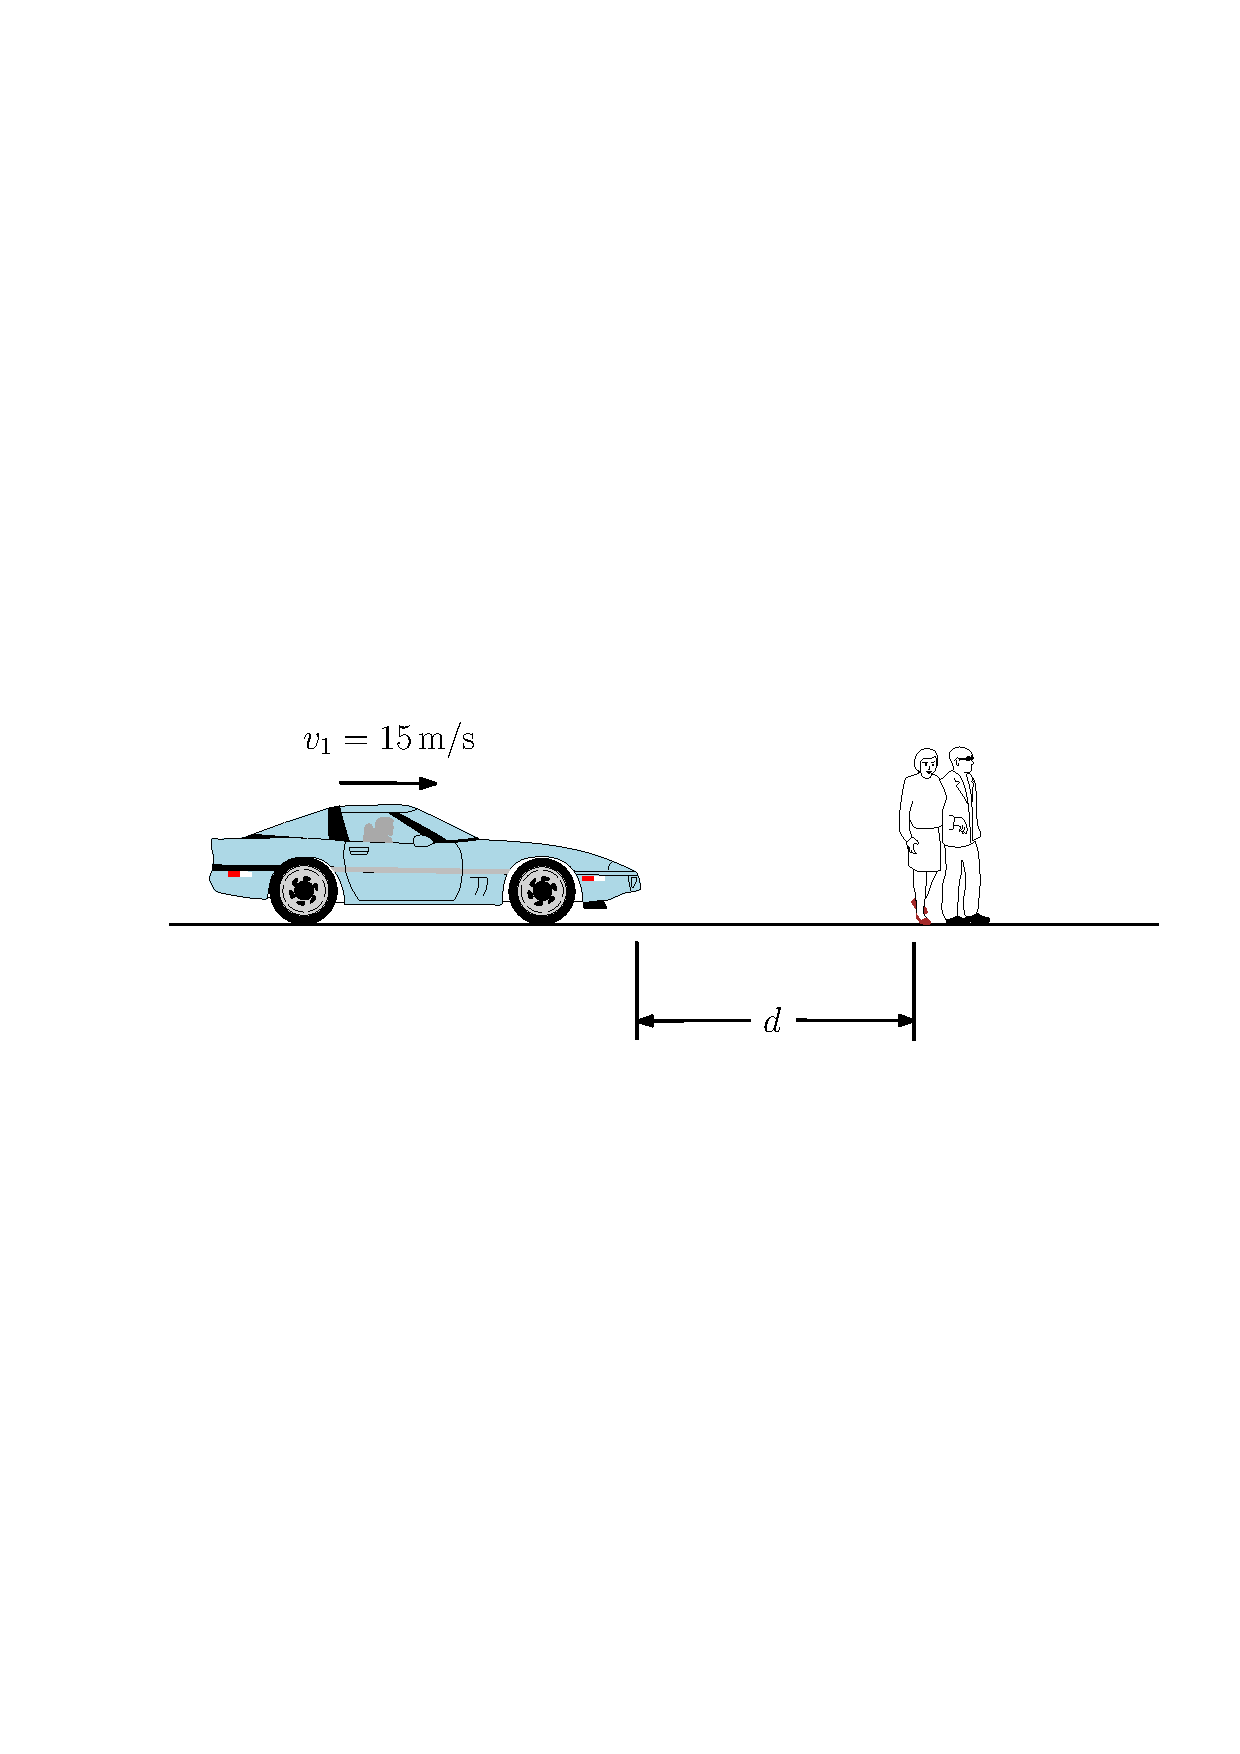
\includegraphics[scale=.7]{images/draw_1.pdf}
		\end{figure}
		
		\textbf{Resposta}
		$
		\begin{cases}
		\text{Motorista normal: } d=\SI{198.75}{\meter}\\
		\text{Motorista com álcool: } d=\SI{232.5}{\meter}
		\end{cases}
		$
		
		\item Se os efeitos da resistência atmosférica são levados em consideração, um corpo caindo tem uma aceleração definida pela equação,
		
		\begin{equation}
		a=9.81\,\big(1-v^{2}\cdot(10^{-4})\big)
		\end{equation}
		
		onde $v$ é dado em \SI{}{\meter/\second} e a direção positiva é para baixo. Se o corpo é solto a partir do repouso a uma altitude muito elevada, determine (a) a velocidade quando $t=\SI{5}{\second}$ e (b) a velocidade máxima possível ou final do corpo (quando $t\rightarrow\infty$)
		
		
		\textbf{Resposta}
		$
		\begin{cases}
		\text{(a) }v=\SI{45.5}{\meter/\second}\\
		\text{(b) }v=\SI{100}{\meter/\second}
		\end{cases}
		$
		
		\item Uma caixa desce deslizando encosta abaixo, como descrito pela equação $y=0.05\,x^{2}$, onde $x$ é dado em metros. Se a caixa tem componente $x$ de velocidade e aceleração $v_{x}=\SI{-3}{\meter/\second}$ e $a_{x}=\SI{-1.5}{\meter/\second^{2}}$ em $x=\SI{5}{\meter}$, determine as componentes $y$ da velocidade e aceleração da caixa neste instante.
		
		\vspace{-.5cm}
		\begin{flushright}
			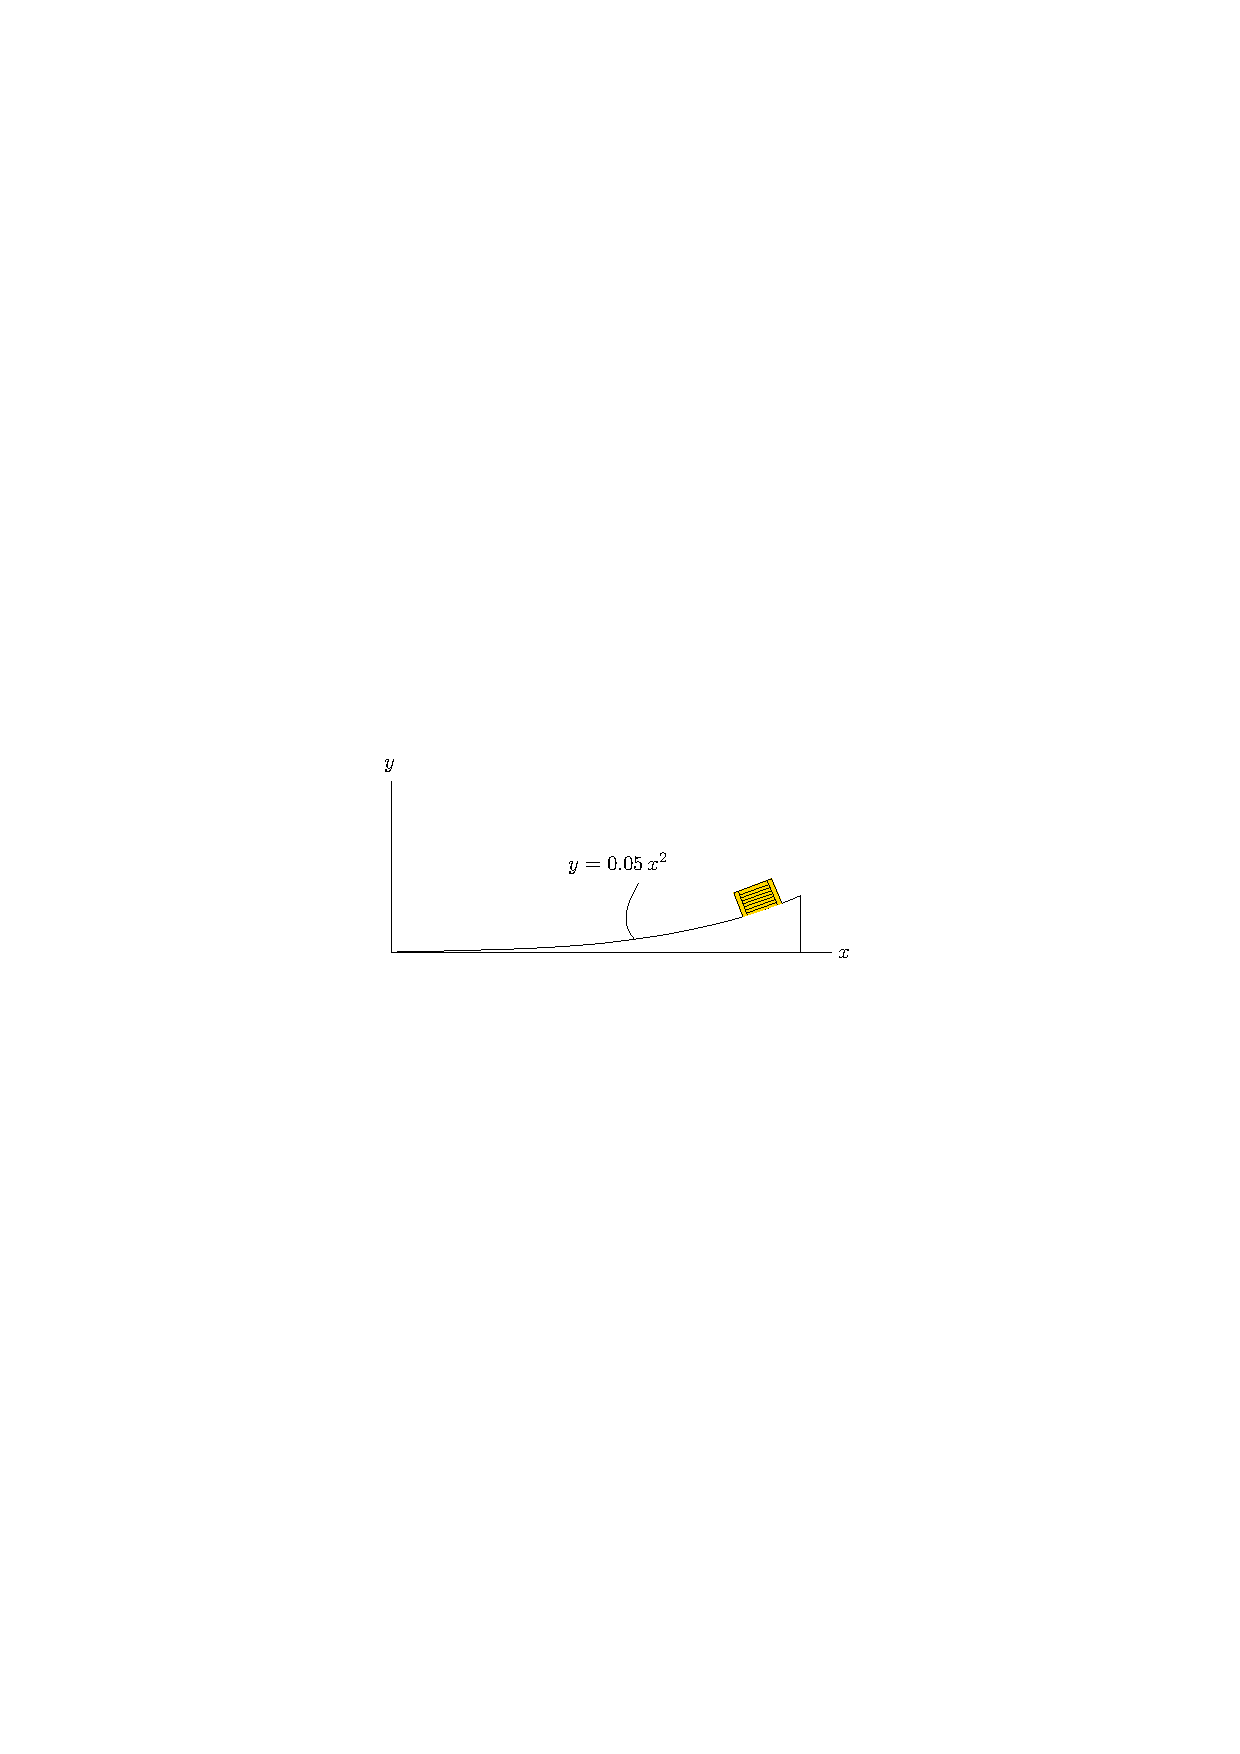
\includegraphics[scale=1.3]{images/draw_2.pdf}
		\end{flushright}
		
		\vspace{-4.35cm}
		\textbf{Resposta}
		$
		\begin{cases}
		v_{y}=\SI{-1.5}{\meter/\second}\\
		a_{y}=\SI{0.15}{\meter/\second^{2}}
		\end{cases}
		$
		
		\vspace{3.5cm}
		\item Uma motocicleta move-se com velocidade escalar constante $v_{0}$ ao longo da trajetória que, por curta distância, assume a forma de uma curva senoidal. Determine as componentes $x$ e $y$ da sua velocidade
		sobre a curva em qualquer instante.
		
		\begin{figure}[h!]
			\centering
			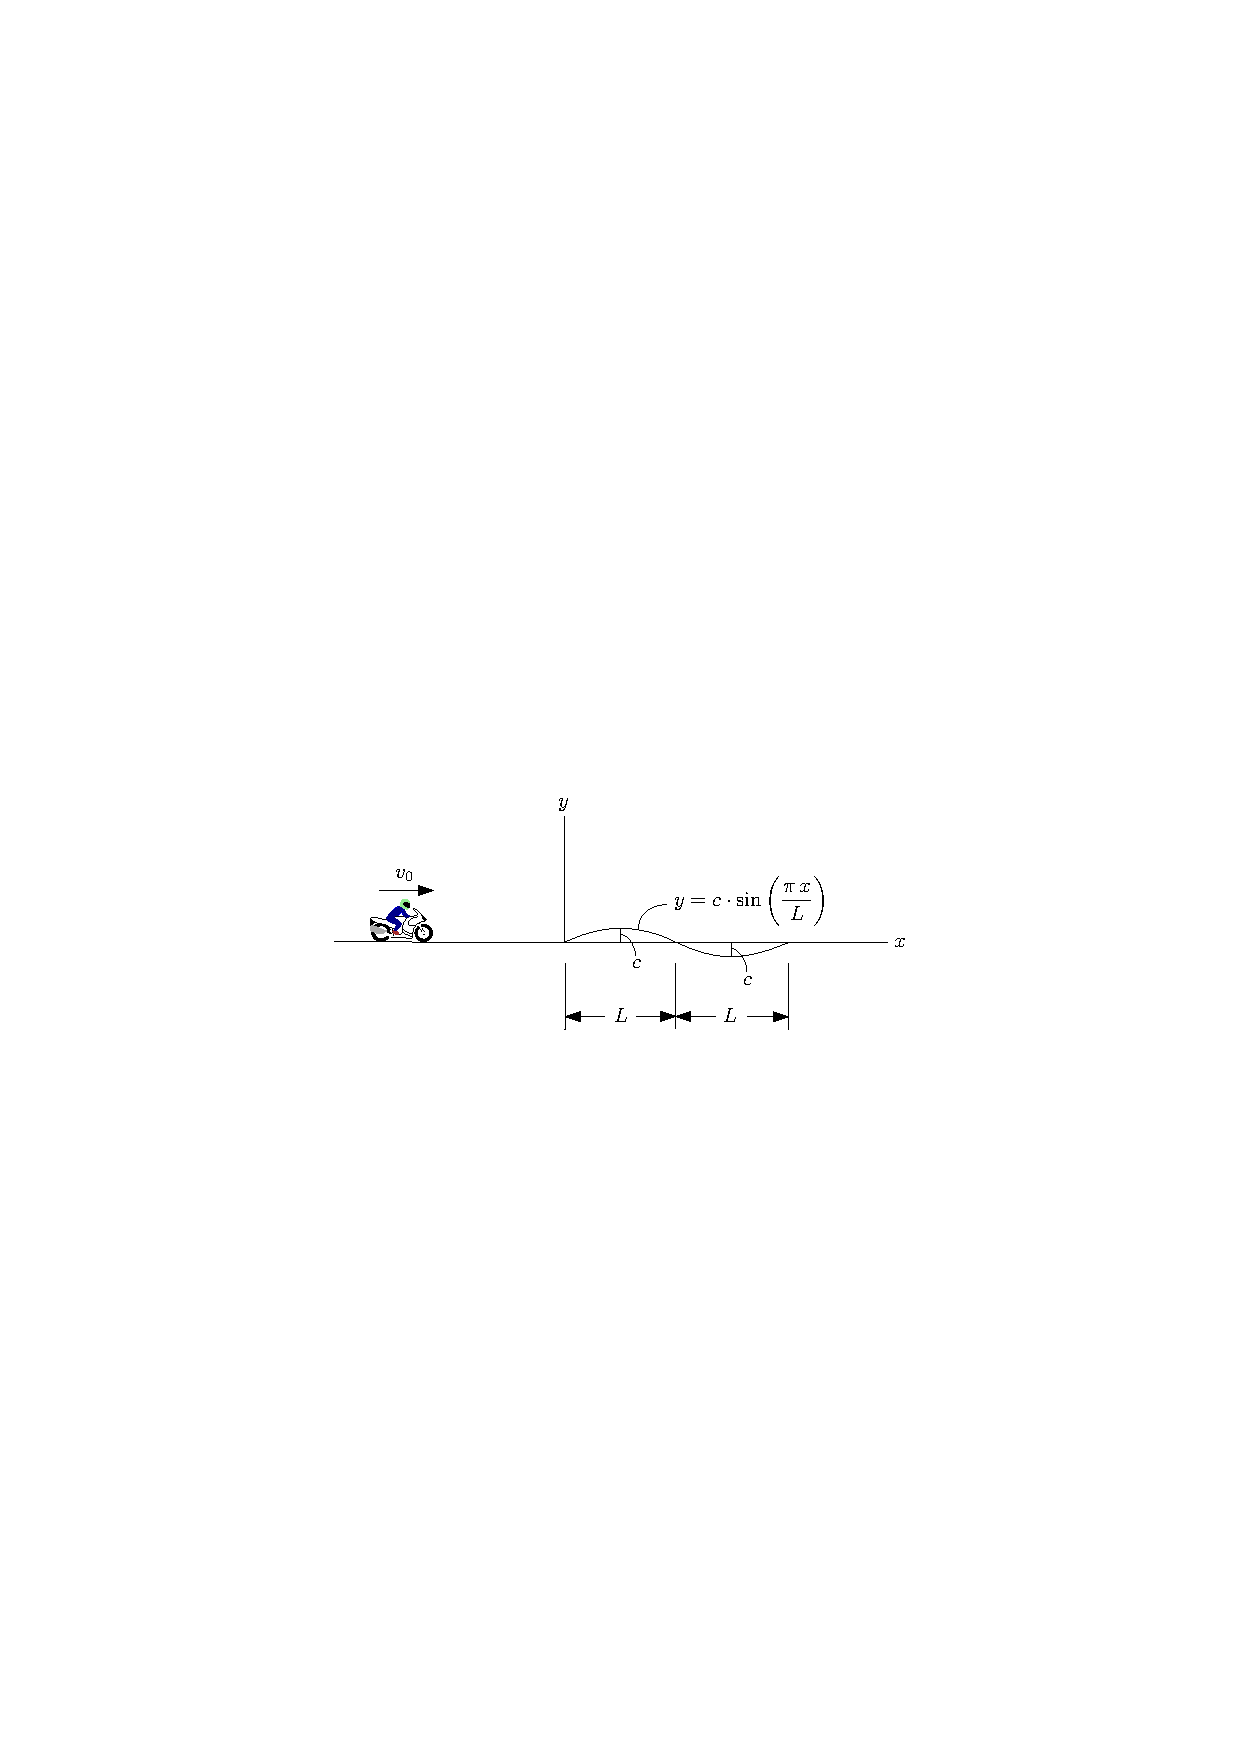
\includegraphics[scale=1.2]{images/draw_3}
		\end{figure}
		
		\textbf{Resposta}
		$
		\begin{cases}
		v_{x}=v_{0}\bigg[1+\bigg(\dfrac{\pi\,c}{L}\bigg)^{2}\cos^{2}\bigg(\dfrac{\pi\,x}{L}\bigg)\bigg]^{-\frac{1}{2}}\\
		v_{y}=\dfrac{v_{0}\,\pi\,c}{L}\bigg(\cos\dfrac{\pi\,x}{L}\bigg)\bigg[1+\bigg(\dfrac{\pi\,c}{L}\bigg)^{2}\cos^{2}\bigg(\dfrac{\pi\,x}{L}\bigg)\bigg]^{-\frac{1}{2}}
		\end{cases}
		$
		
		
		\item Uma bola de futebol americano é chutada sobre o poste do gol com velocidade inicial de $v_{A}=\SI{24}{\meter/\second}$ como mostrado. Determine o ponto $B=(x,y)$ onde ela atinge as arquibancadas.
		
		\textbf{Resposta}
		$
		\begin{cases}
		t=\SI{2.937}{\second}\\
		y=x=\SI{18.74}{\meter}
		\end{cases}
		$
		\vspace{-1cm}
		\begin{flushright}
			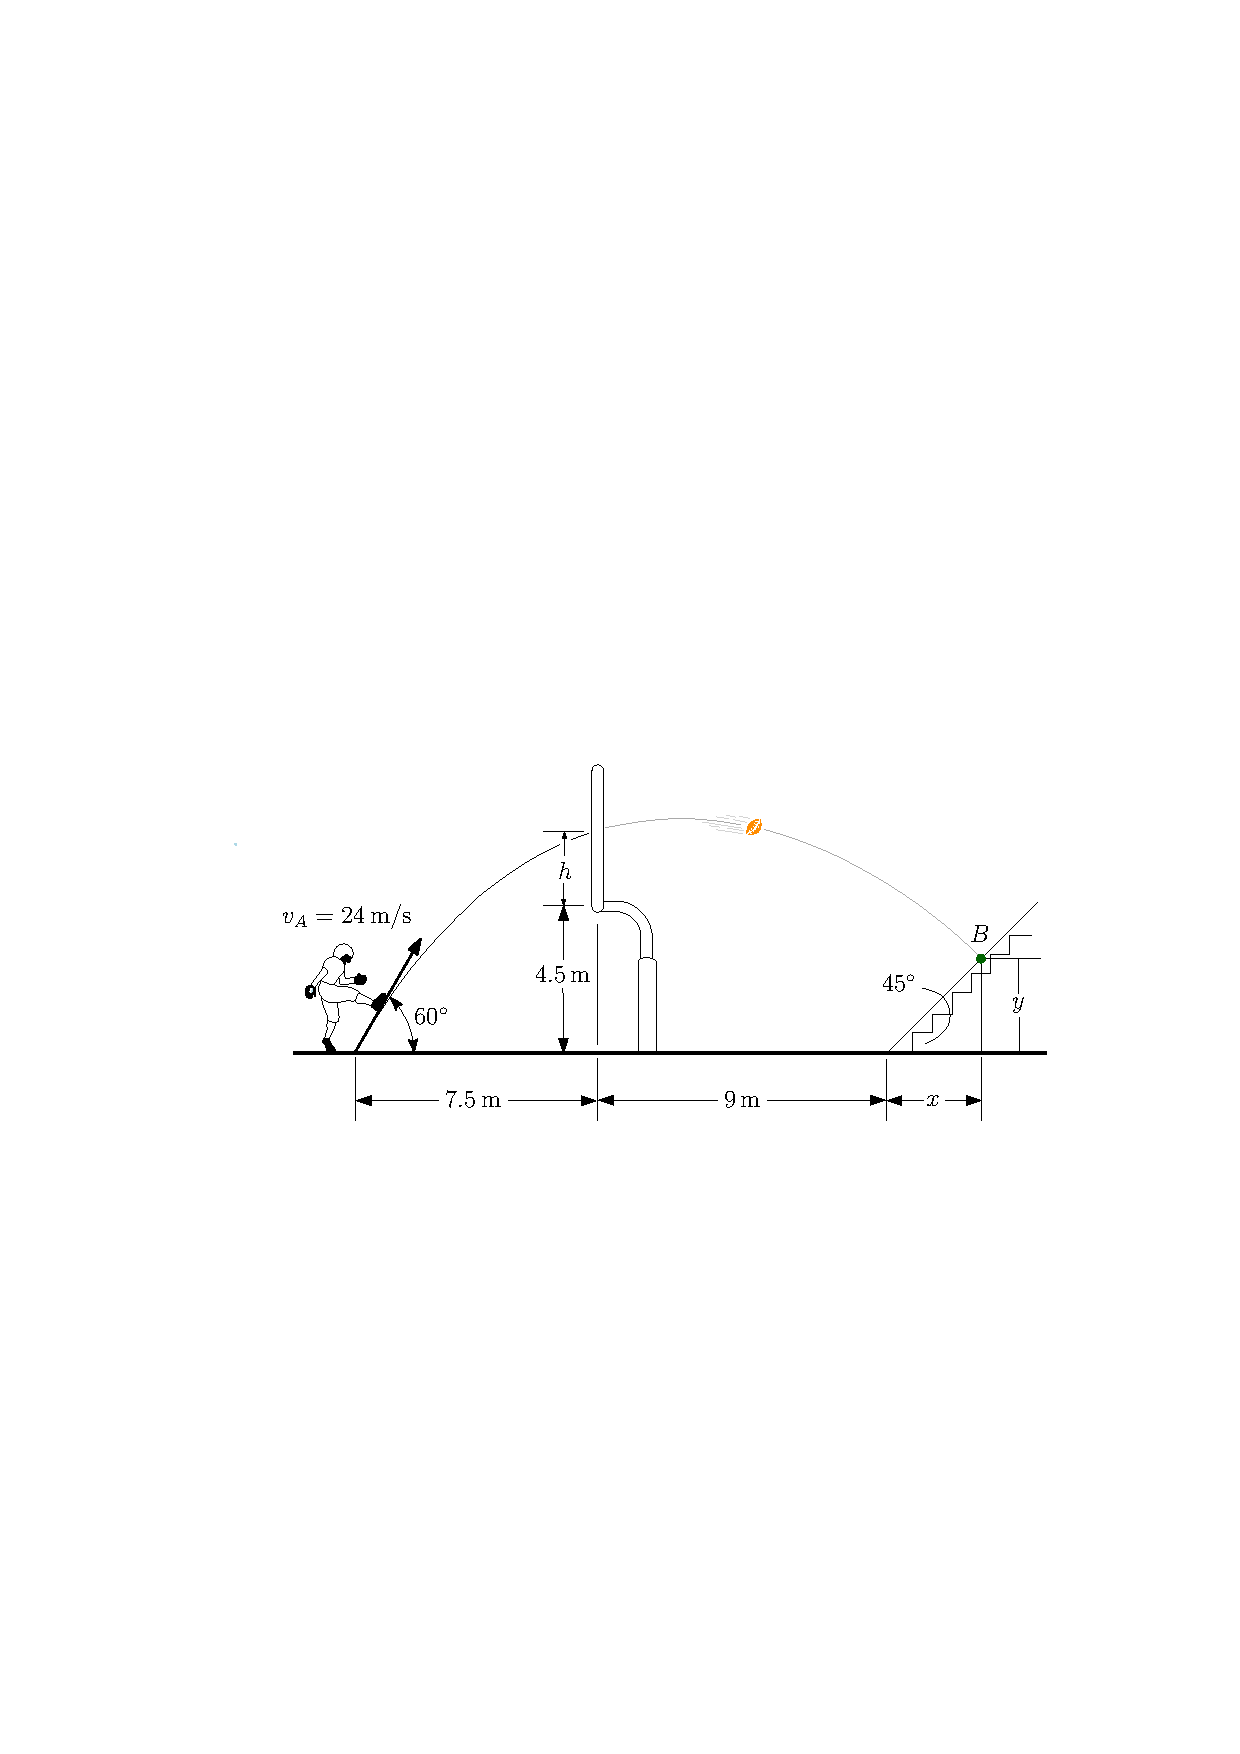
\includegraphics[scale=1.1]{images/draw_10}
		\end{flushright}
		
		\newpage
		
		
		\item O carro de corrida move-se com velocidade escalar constante de \SI{240}{\kilo\meter/\hour} em torno da pista elíptica. Determine a aceleração sentida pela motorista em $B$.
		
		\vspace{-.5cm}
		\begin{flushright}
			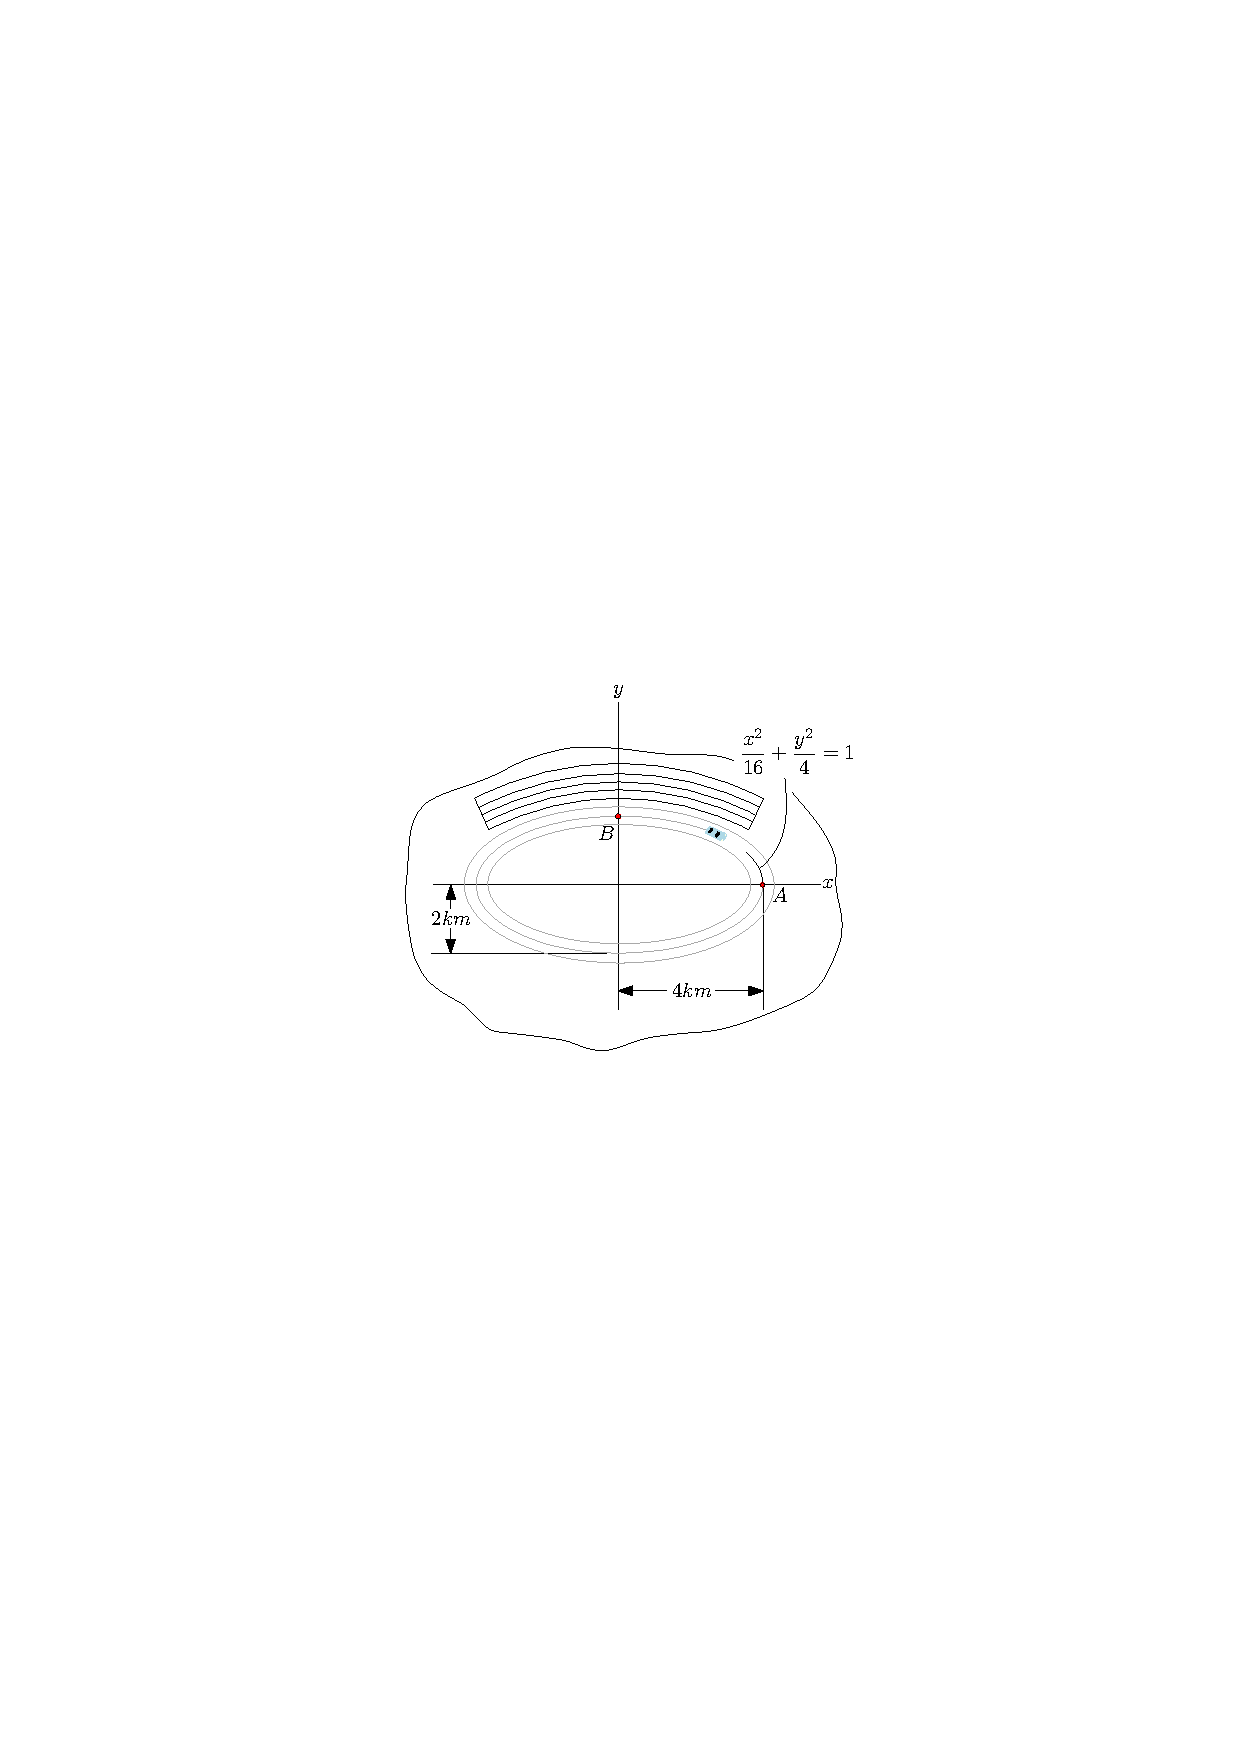
\includegraphics[scale=1.2]{images/draw_4}
		\end{flushright}
		
		\vspace{-8.5cm}
		$\textbf{\text{Resposta}}\Rightarrow a=\SI{0.556}{\meter/\second^{2}}$
		\vspace{7.5cm}
		
		\item Um motociclista desloca-se ao longo da curva a uma velocidade escalar constante de \SI{9}{\meter/\second}. Determine a sua aceleração quando ele está localizado no ponto $A$. Despreze a dimensão da motocicleta e do motociclista para o cálculo.
		
		\begin{flushleft}
			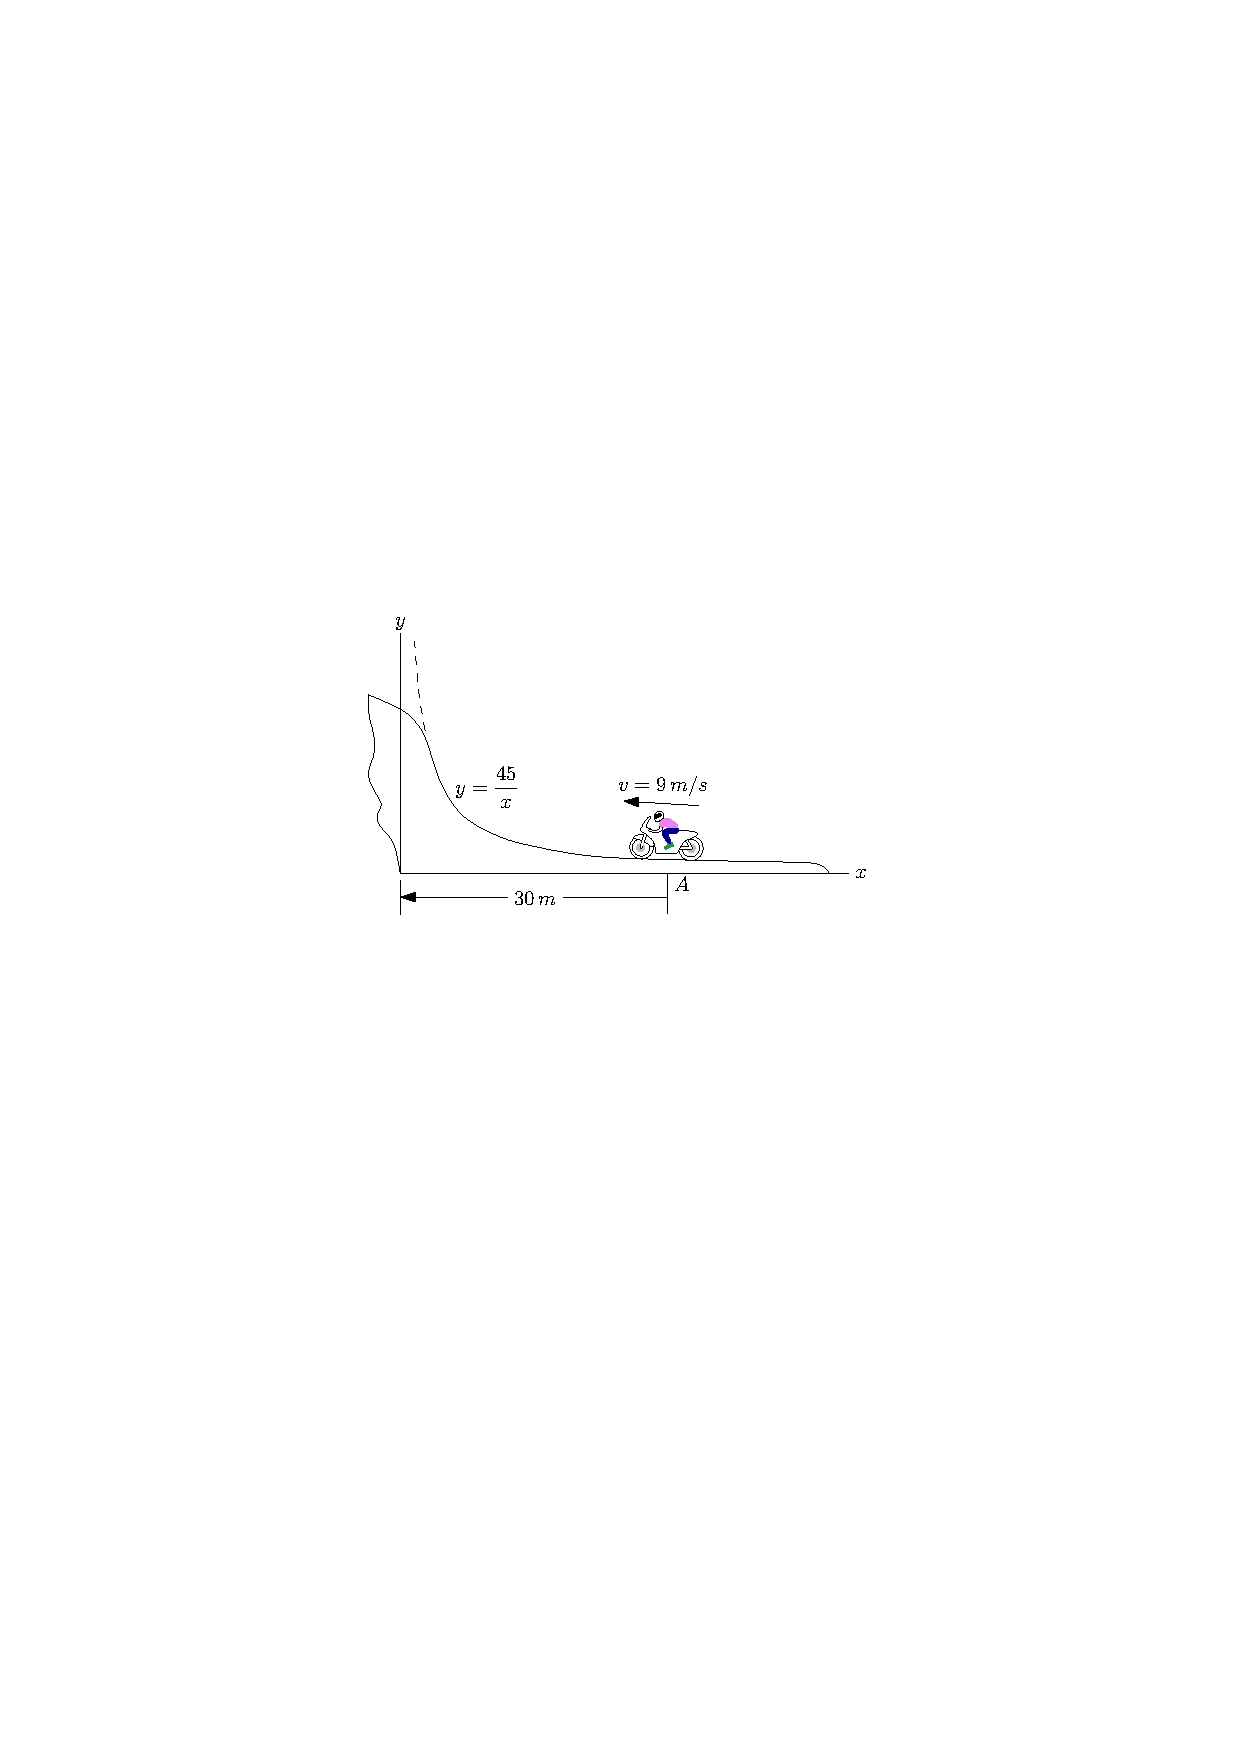
\includegraphics[scale=1.2]{images/draw_5}
		\end{flushleft}
		
		\vspace{-8cm}
		\begin{flushright}
			$\textbf{\text{Resposta}}\Rightarrow	a=\SI{0.269}{\meter/\second^{2}}$
		\end{flushright}
		\vspace{5.7cm}
		
		\item O movimento do pino $P$ é restringido pela fenda curva da lemniscata em $OB$ e pela fenda do braço $AO$. Se $AO$ gira no sentido anti-horário com uma velocidade angular $\dot{\theta}=3\,t^{3/2}[\SI{}{\radian/\second}]$, onde $t$ é dado em segundos, determine as intensidades da velocidade e aceleração do pino $P$ em $\theta=30^{\circ}$. Sabe-se que em $t=0$, $\theta=0^{\circ}$
		
		\vspace{-.5cm}
		\begin{flushright}
			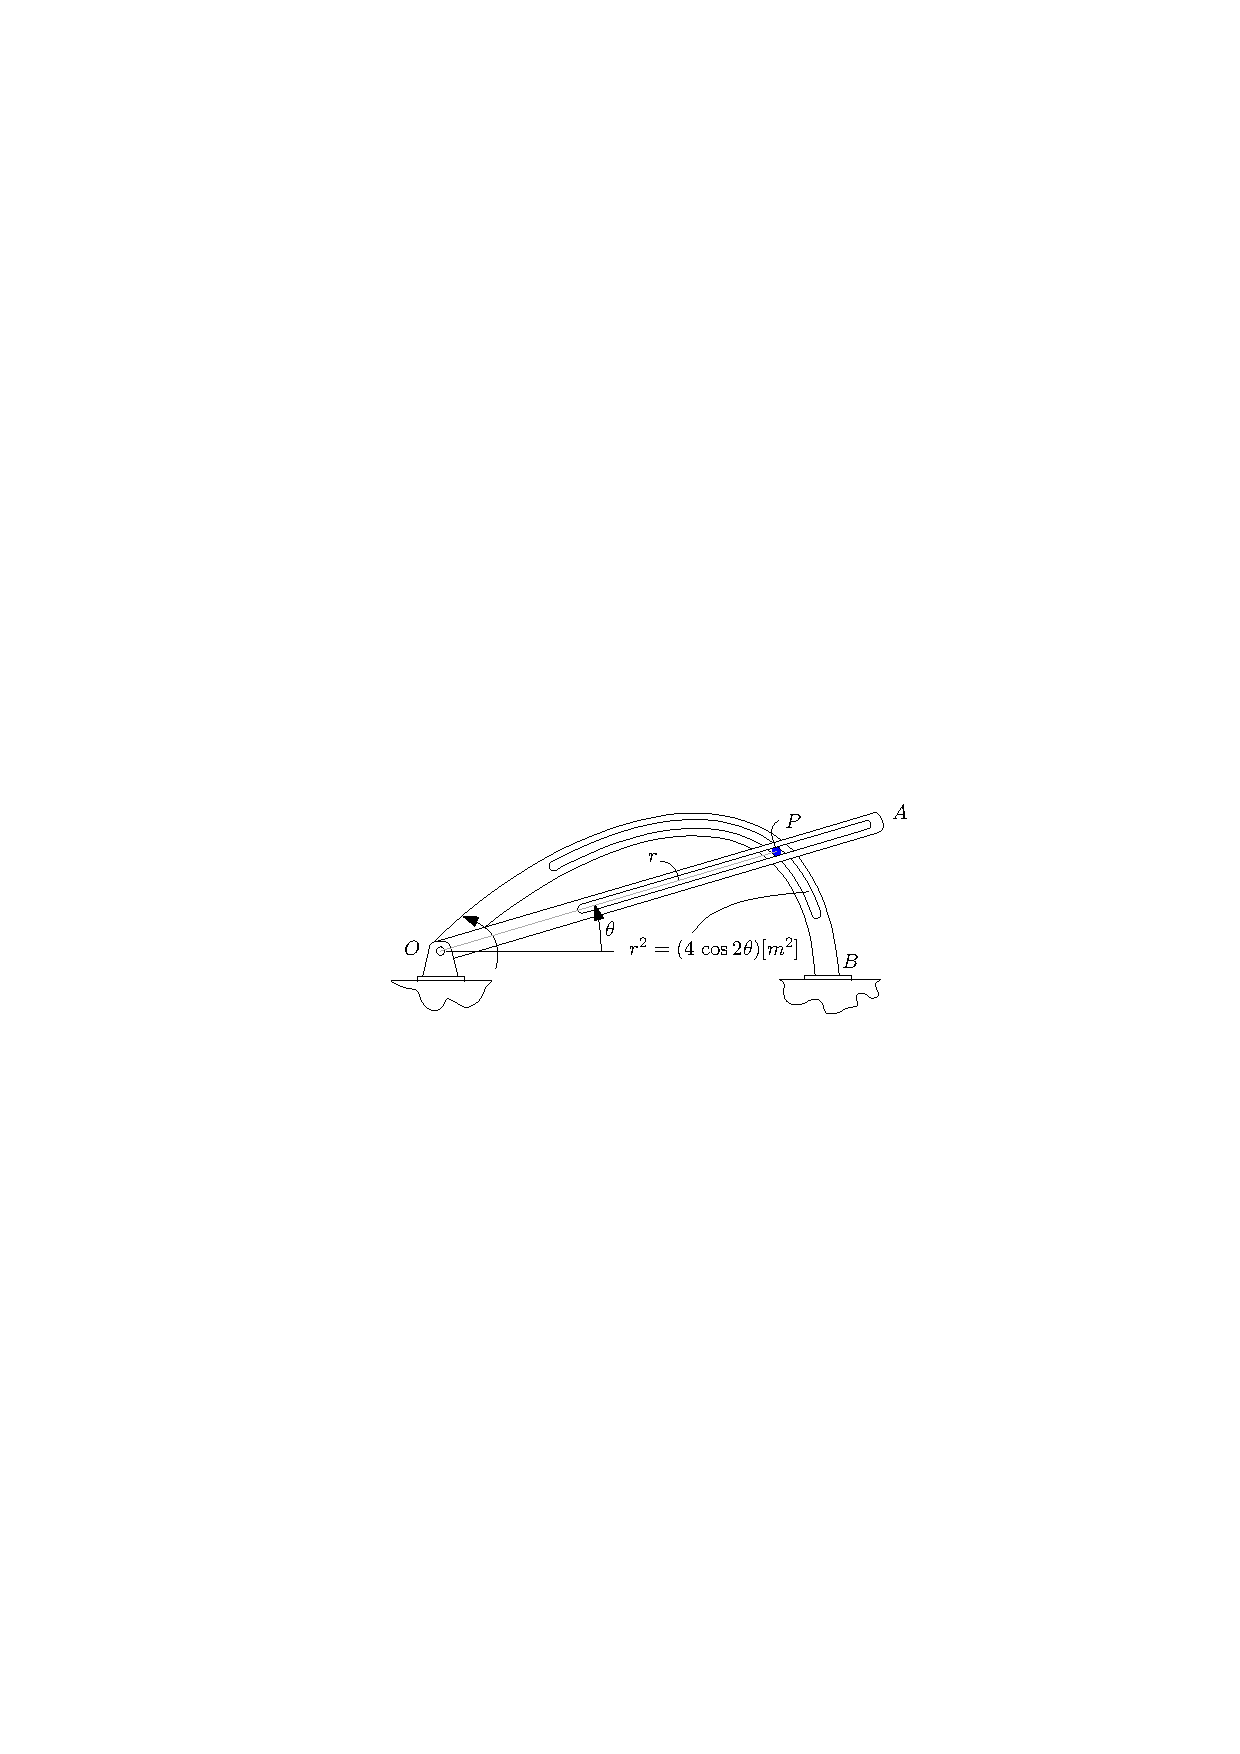
\includegraphics[scale=1.2]{images/draw_6}
		\end{flushright}
		
		\vspace{-4.8cm}
		\textbf{Resposta}
		$
		\begin{cases}
		v=\SI{5.16}{\meter/\second}\\
		a=\SI{39.1}{\meter/\second^{2}}
		\end{cases}
		$
		
		\newpage
		\item Um barco move-se ao longo de uma trajetória definida por $r^{2}=0.9\cdot 10^{3}\cdot\cos 2\theta\,[\,\SI{}{\meter}^{2}\,]$, onde $\theta$ é dado em radianos. Se $\theta=0.4\,t^{2}$, onde $t$ é dado em segundos, determine as componentes radiais e transversais da velocidade e aceleração do barco no instante $t=\SI{1}{\second}$
		
		\begin{flushright}
			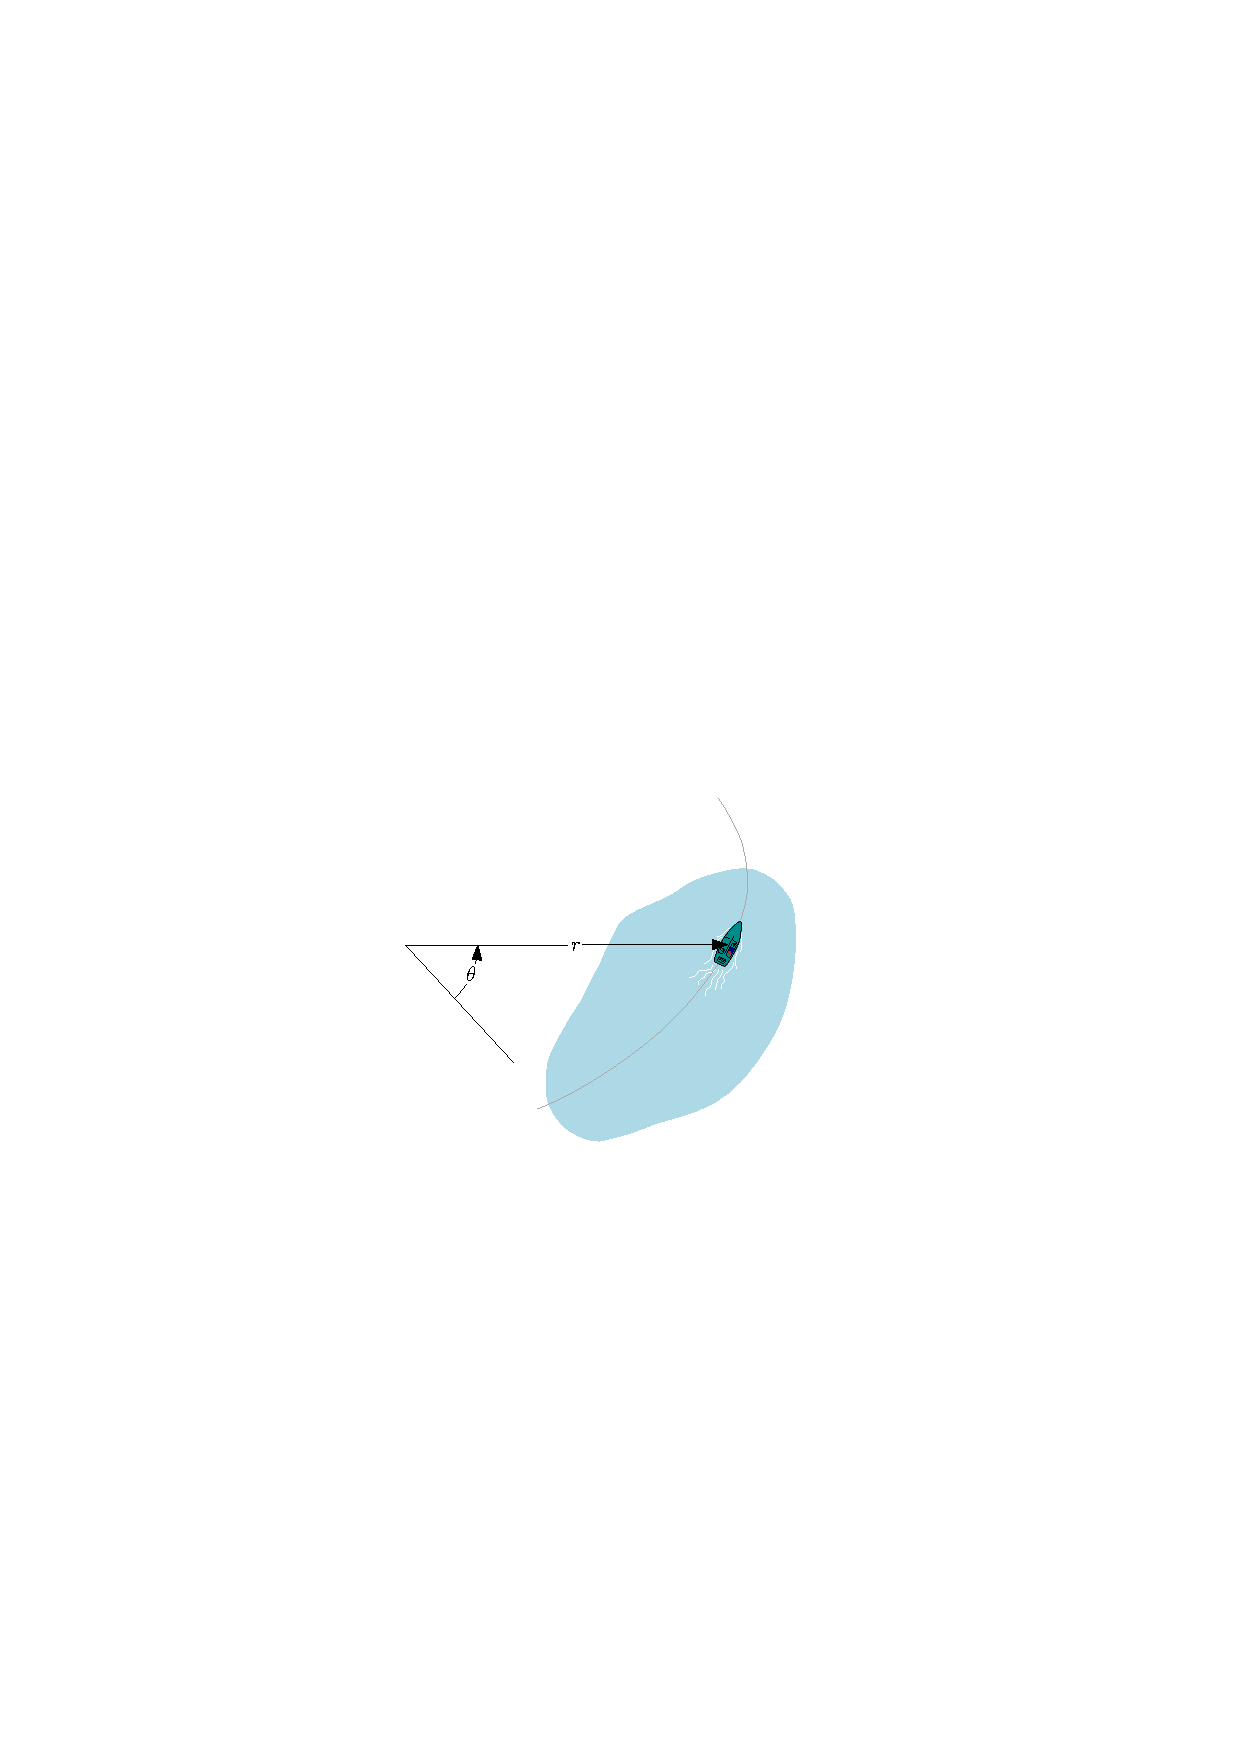
\includegraphics[scale=1.35]{images/draw_7.pdf}
		\end{flushright}
		
		\vspace{-10.5cm}
		\textbf{Resposta}
		$
		\begin{cases}
		v=\dot{r}=\SI{-20.63}{\meter/\second}\\
		v=r\,\dot{\theta}=\SI{20}{\meter/\second}\\
		a=\ddot{r}-r\,\dot{\theta}^{2}=\SI{-85.7}{\meter/\second^{2}}\\
		a=r\,\ddot{\theta}+2\,\dot{r}\,\dot{\theta}=\SI{-12.98}{\meter/\second^{2}}
		\end{cases}
		$
		\vspace{7cm}

		\item Se a corda é puxada na direção do motor $M$ com uma velocidade escalar $v=5\,t^{\frac{3}{2}}\,[\SI{}{\meter/\second}]$, onde $t$ é dado em segundos, determine a velocidade escalar do cilindro $A$ quando $t=\SI{1}{\second}$ 
		
		
		\begin{flushright}
			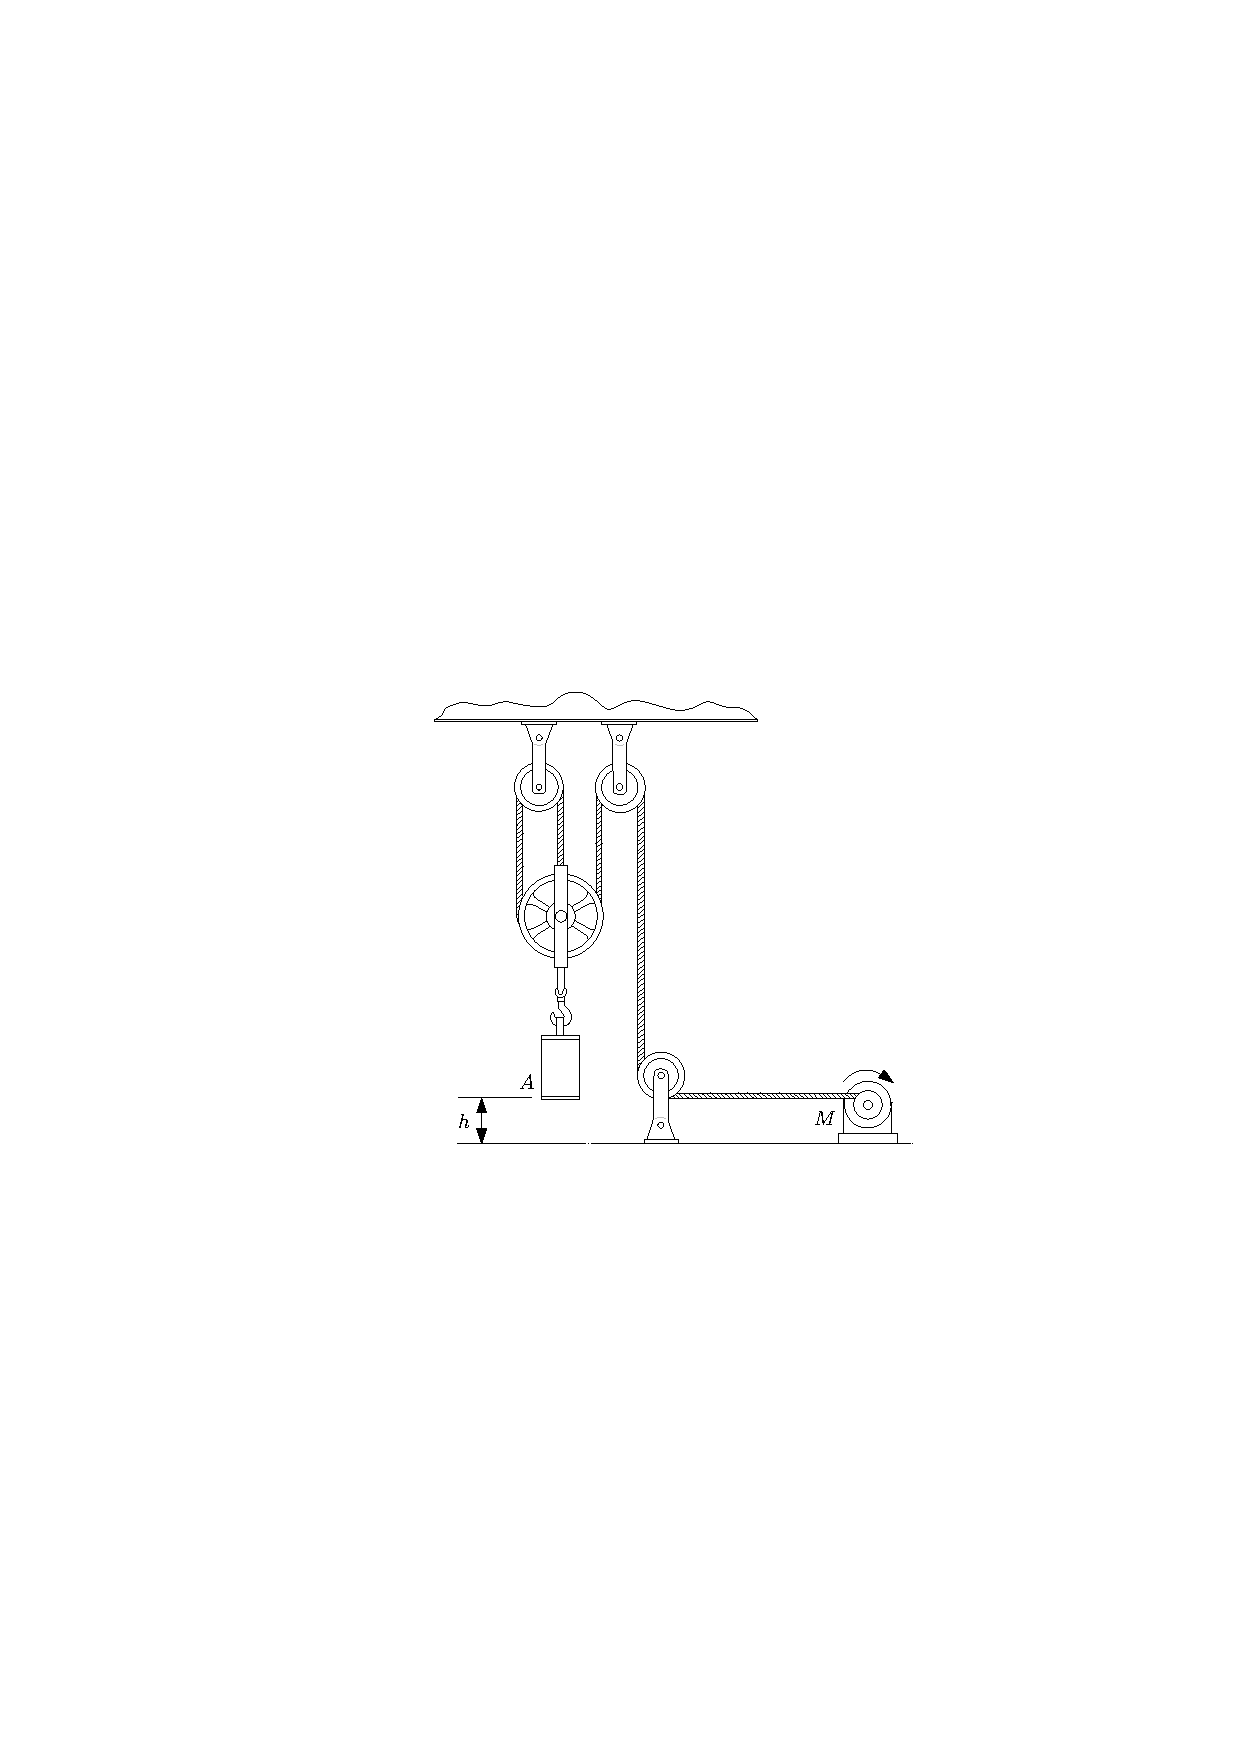
\includegraphics[scale=1.3]{images/draw_8}
		\end{flushright}
		
		\vspace{-11.7cm}
		$\textbf{\text{Resposta}}\Rightarrow	v=\SI{1.67}{\meter/\second}$
		
		\newpage
		\item Se a extremidade do cabo $A$ é puxada para baixo com uma velocidade escalar de $\SI{2}{\meter/\second}$ determine a velocidade escalar na qual o bloco $E$ sobe.
		
		$\textbf{\text{Resposta}}\Rightarrow	v=\SI{0.250}{\meter/\second}$
		
		\vspace{-1cm}
		\begin{flushright}
			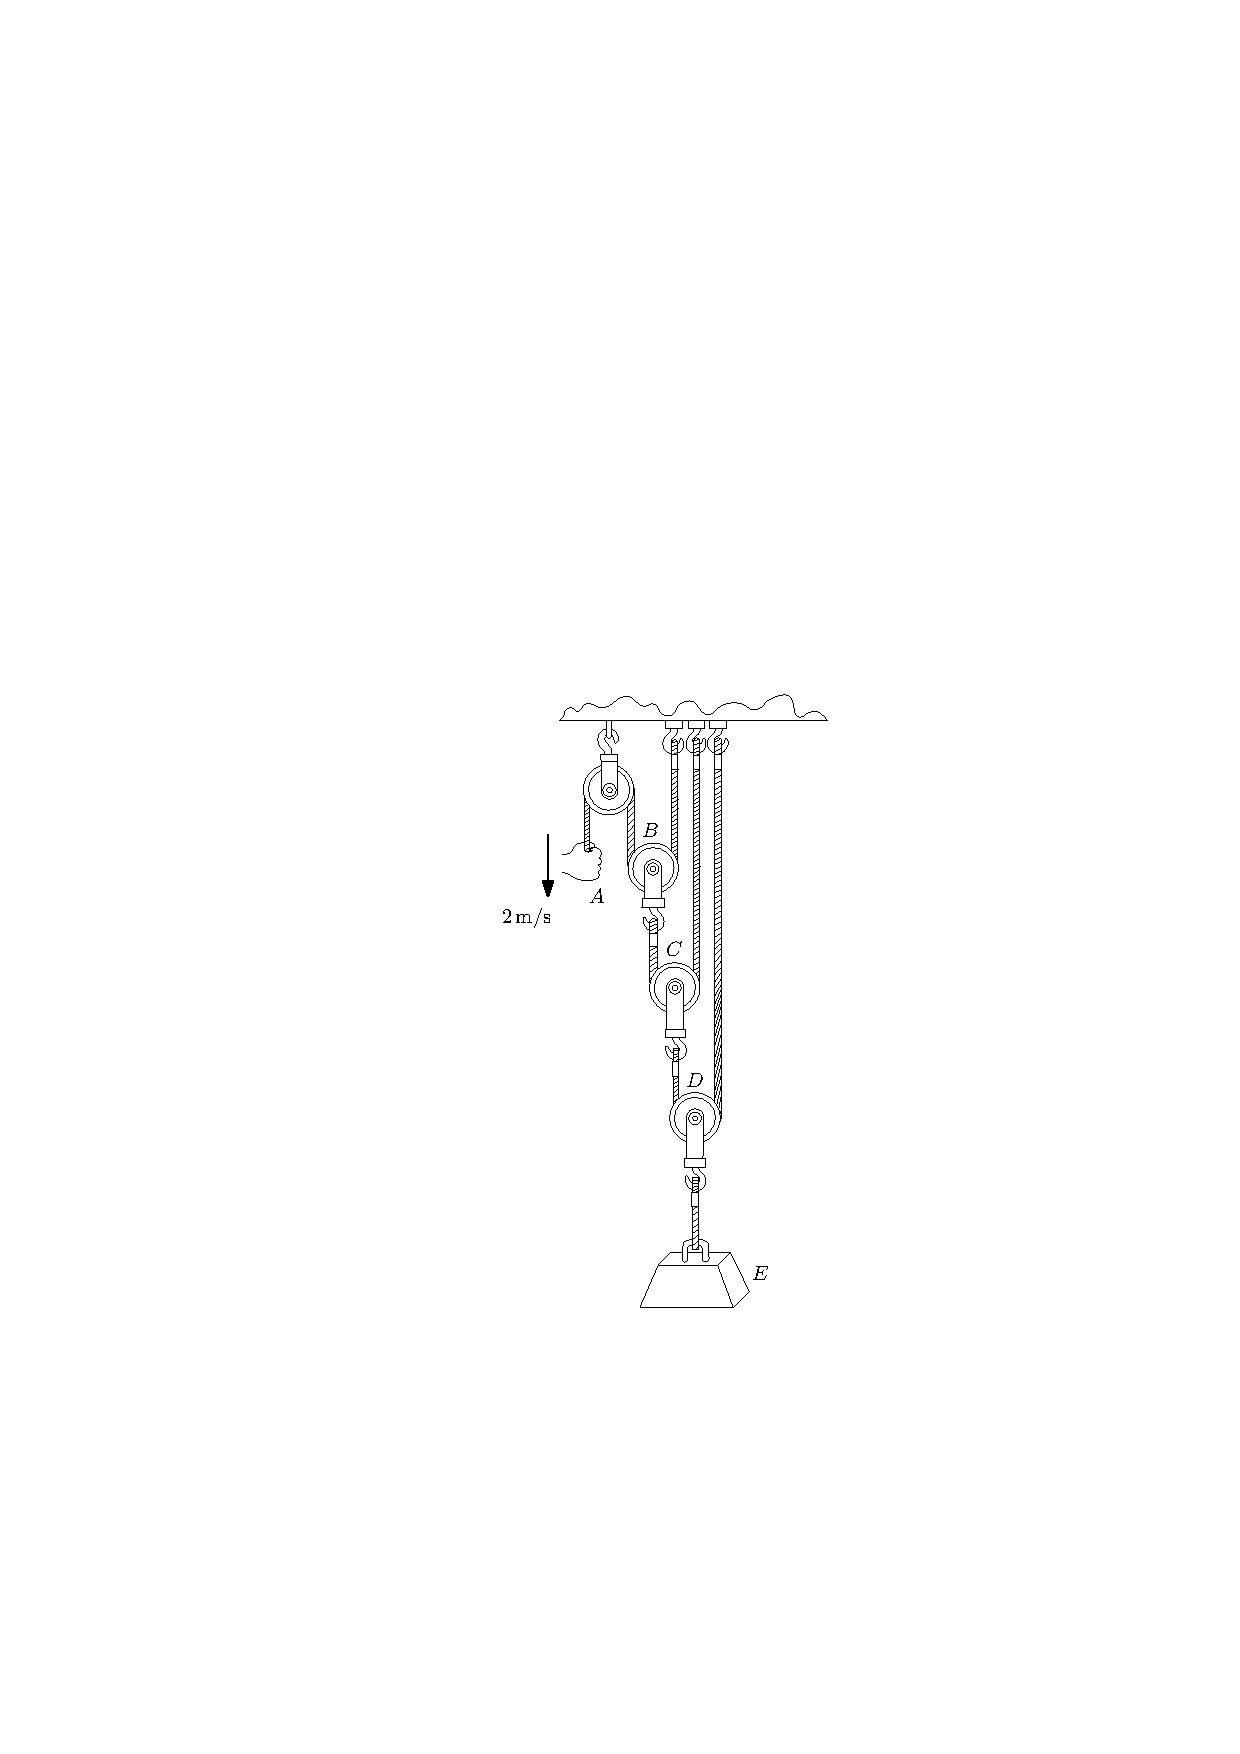
\includegraphics[scale=1.3]{images/draw_9}
		\end{flushright}
		
		
	\end{enumerate}
\end{document}